\chapter{Bewertung des Prototyps}
In diesem Kapitel wird der entwickelte Prototyp zunächst mit dem traditionellen, analogen Prozess der Aufmaßerfassung bzgl. der Effizienz vergleichen.
Anschließend werden Probleme und Grenzen aufgezeigt, die sich während des Entwicklungsprozesses identifizieren lassen haben.

\section{Vergleich mit analoger Aufmaßerfassung}
Zum Zeitpunkt dieses Vergleiches (5. März 2018) ist der finale Prototyp bereits seit Ende Januar unternehmensweit in die vorhandene Android-App eingebunden.
Da die Bilder, welche über den Prototyp aufgenommen und hochgeladen werden, mit der Kategorie ``measurement'' markiert werden, kann genau nachvollzogen werden, wie viele Bilder von welchem Angestellten mit Hilfe des Prototyps aufgenommen wurden. \\

Am Standort in Bulgarien wurden im Zeitraum vom 31. Januar bis 2. März insgesamt zwölf Bilder von zwei verschiedenen Benutzern über den eingebundenen Prototyp hochgeladen (vgl. \autoref{fig:usagebg}).
Sieben dieser Bild stammen von einer der Testpersonen (André Vermeulen) und die restlichen fünf von einem der bulgarischen Angestellten.
Dieser Mitarbeiter hat es geschafft, ohne jegliche externe Hilfestellung die Funktion zur Aufmaßerfassung innerhalb der bestehenden App zu finden, ein Bild zu importieren, dieses zu bearbeiten und anschließend das bearbeitete Bild hochzuladen. \\

Am Standort Paderborn wurde der eingebundene Prototyp fast doppelt so häufig genutzt wie in Bulgarien.
Hier wurden in der Zeitspanne vom 25. Januar bis 27. Februar insgesamt 20 annotierte Bilder von fünf verschiedenen Benutzern aufgenommen und hochgeladen (vgl. \autoref{fig:usagepb}).
Diese fünf Benutzer setzen sich aus den beiden Testpersonen und drei weiteren Mitarbeitern zusammen, die ohne jegliche Aufforderung oder Hilfestellung auf die Funktion des Prototyps aufmerksam geworden sind und diesen nur mit den im Prototyp vorhandenen Hilfe-Overlays bedient haben. \\

Auch für das Fassadengerüst, welches bereits in \autoref{sec:problem} vorgestellt wurde, wurden mit Hilfe des Prototyps Aufmaße erstellt (siehe \autoref{fig:comparison}).
Das annotierte Bild (\autoref{fig:new}) wirkt im Vergleich zur handschriftlichen Aufmaßerfassung in \autoref{fig:old} übersichtlicher und verständlicher, da dem Betrachter durch das Bild des Gerüsts mehr Kontext zur Verfügung gestellt wird als mit der handschriftlichen Skizze. \\

\begin{figure}[h]
  \begin{subfigure}[t]{0.4\textwidth}
    \centering
    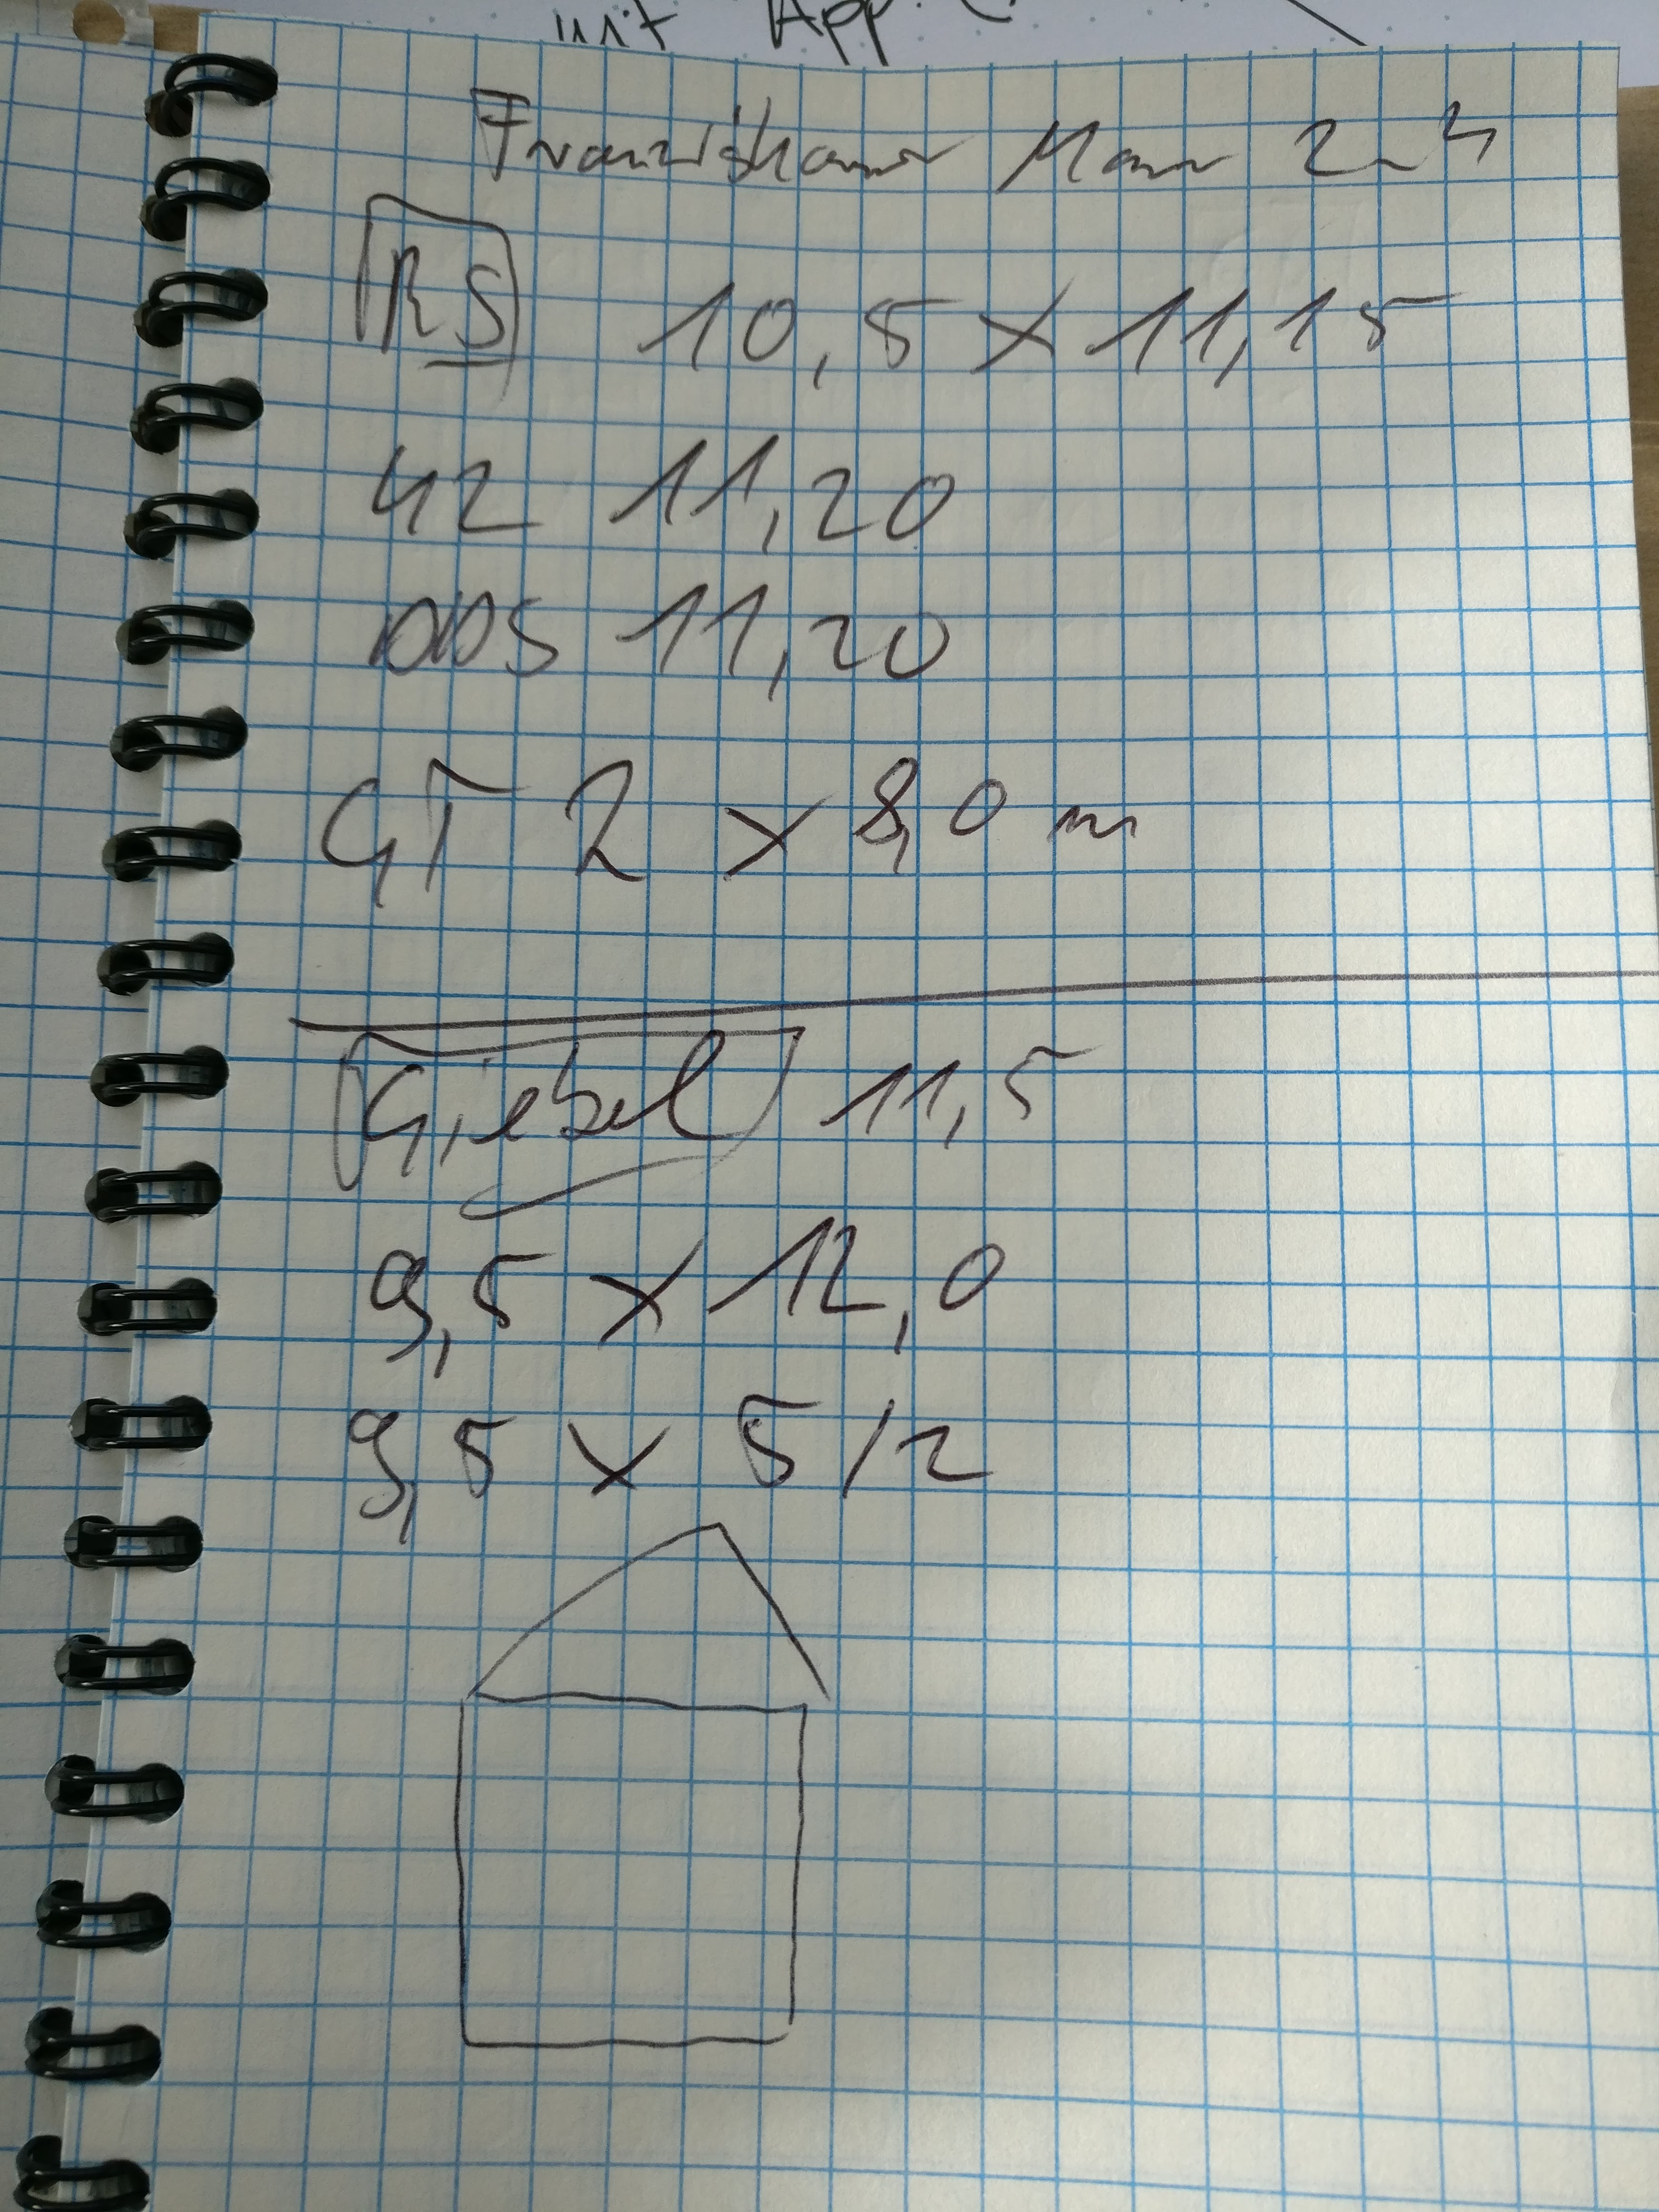
\includegraphics[keepaspectratio, height=\textwidth]{aufmasse/notes}
    \caption{Handschriftliche Aufmaße des Fassadengerüst}
    \label{fig:old}
  \end{subfigure}
  ~
  \begin{subfigure}[t]{0.4\textwidth}
    \centering
    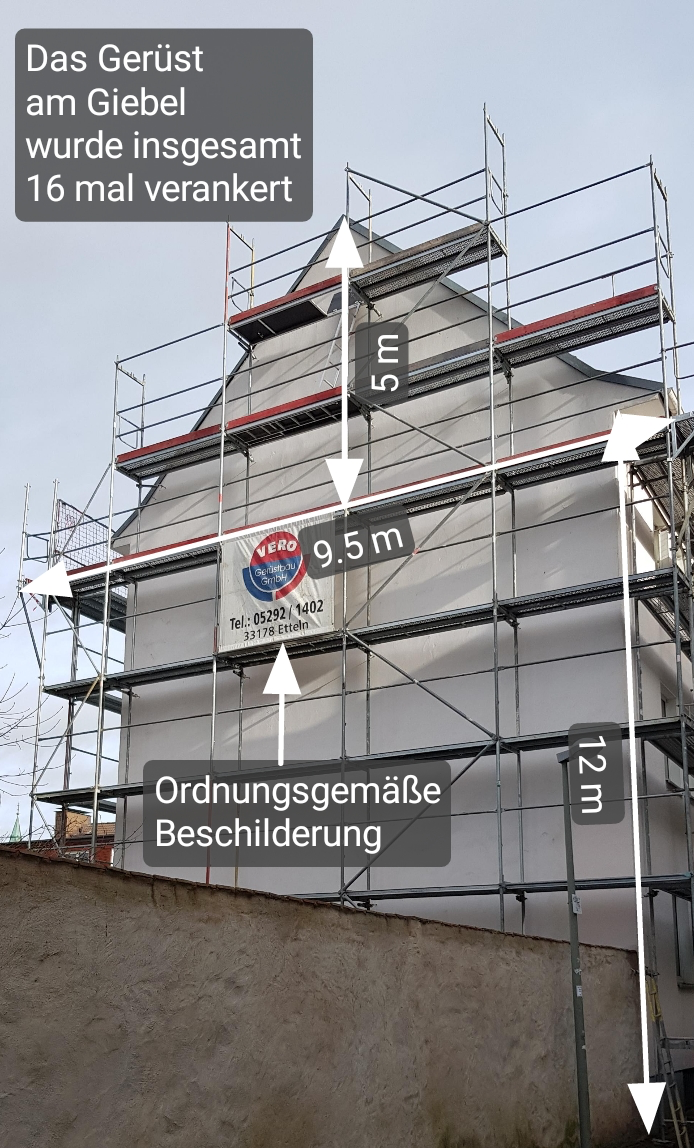
\includegraphics[keepaspectratio, width=0.75\textwidth]{data/annotated}
    \caption{Mit Hilfe der App annotiertes Bild des Fassadengerüsts}
    \label{fig:new}
  \end{subfigure}
  \centering
  \caption{Handschriftliche und digitale Aufmaßerfassung des Fassadengerüsts}
  \label{fig:comparison}
\end{figure}

Zusammenfassend kann festgehalten werden, dass der Prototyp zur mobile Aufmaßerfassung bereits von einigen Mitarbeitern selbstständig entdeckt und benutzt wurde.
Trotz der nicht IT-affinen Zielgruppe ist es diesen Mitarbeitern gelungen, die App ohne externe Hilfestellungen zu bedienen.
Dies spricht für eine intuitiv gestaltete Oberfläche und eine gute Umsetzung der Usability-Kriterien aus \autoref{chap:eval}.
Im Vergleich zum traditionellen, analogen Prozess der Aufmaßerfassung ist der digitale Prozess mit Hilfe der App zeitaufwändiger.
Hier ist die Anfertigung einer handschriftlichen Skizze des Gerüstes tendenziell schneller umsetzbar als das Aufnehmen und Beschriften eines Bildes.
Erst in der nachgelagerten Arbeit wird die Effizienz des digitalen Ansatzes mit Hilfe der App deutlich.
Wobei eine handschriftliche Skizze nicht direkt für alle Mitarbeiter verfügbar ist, ist das annotierte Bild direkt im System vorhanden, nachdem es hochgeladen wurde.
Zudem wird durch die App das Problem gelöst, dass gesammelte Daten durch unverständliche Notizen nur vom ursprünglichen Verfasser zu lesen sind oder verloren gehen, noch bevor sie ins System eingetragen werden konnten.

\section{Probleme und Grenzen}
Während des Entwicklungsprozesses der App haben sich verschiedene Usability-Probleme gezeigt, die in den einzelnen Zyklen des \hcdp{} gelöst wurden.
Jedoch gab es auch Probleme, die mit Hilfe der Android-App nicht gelöst werden konnten.
In diesem Kapitel werden die Probleme und Grenzen der mobilen Bildbearbeitung zur Aufmaßerfassung im Gerüstbau näher beleuchtet. \\

Die Verdeckung des zu beaufmaßenden Gerüsts durch ein Hindernis wurde während der Aufmaßerfassung des Gebäudes in \autoref{sec:problem} als Problem deutlich.
Hier wurde eine Seite des Gebäudes von einem Baum so verdeckt, dass mit Hilfe der App nur schwer ein verwendbares Bild aufgenommen werden konnte.
In diesem Fall konnte durch die Veränderung des Aufnahmewinkels trotzdem ein Bild der Gebäudeseite aufgenommen werden.
Jedoch ist eine solche Anpassung des Aufnahmewinkels nicht immer ohne Weiteres möglich.
Insbesondere bei Gebäuden, die nah zusammen stehen oder nur aus einem eingeschränkten Aufnahmewinkel fotografiert werden können, ist dies ein Problem, welches durch die Nutzung der App nicht gelöst werden konnte. \\

Der eingeschränkte Aufnahmewinkel des Bildes ist ein weiteres Problem, das während der Aufmaßerfassung des Gebäudes in \autoref{sec:problem} deutlich wurde und nicht mit Hilfe der Android-App gelöst werden konnte.
Besonders bei Gebäudeseiten, die bspw. zu einer Gasse ausgerichtet sind, ist die Aufnahme der gesamten Gebäudeseite nur schwer möglich.
Um trotzdem ein Bild der gesamten Gebäudeseite aufzunehmen, muss der Nutzer das Bild aus einem spitzen Winkel aufnehmen.
Hierdurch können einerseits Verzerrungen des Bildes entstehen, wodurch Längen optisch anders wahrgenommen werden.
Andererseits kann es passieren, dass für die Aufmaßerfassung wichtige Details aus diesem Aufnahmewinkel nicht zu erkennen sind.
